\section{Memory functions and physical substrates}\label{sec:C14:taxonomy}
Agent memory is a collection of mechanisms for preserving, transforming, locating, and applying information across decisions. Working memory describes the task-relevant information currently available for control. Episodic memory preserves contextualized experience, including what was attempted, observed, and concluded in a particular situation. Semantic memory represents more reusable propositions or abstractions. These are functional distinctions. A vector database can store episodes or semantic statements, and one text document can contain both. The storage technology does not determine the memory function.

Biological terminology can motivate questions about consolidation, salience, interference, and forgetting, but it does not establish a shared implementation. A transformer context is not a demonstrated model of human working memory, and a graph of extracted facts is not a biological semantic system. Parametric knowledge, key-value caches, external records, and application state have different update and access mechanisms. The memory surveys provide useful taxonomies of forms, functions, and dynamics while also revealing how heterogeneous the underlying mechanisms are~\cite{corpus251213564,corpus260206052}.

Represent a memory object as
\begin{equation}
 m=(x,k,p,\tau_v,\tau_o,\sigma,\omega,v),
\end{equation}
where $x$ is content, $k$ its functional type, $p$ provenance, $\tau_v$ valid time, $\tau_o$ observation time, $\sigma$ confidence or status, $\omega$ ownership and access scope, and $v$ its version. This schema is proposed synthesis. It is deliberately richer than an embedding and text pair because future decisions can depend on whether a record is a direct observation, a tentative inference, or an obsolete preference. Embedding proximity alone does not supply those distinctions.

Working context should contain selected memory objects and the metadata needed to interpret them. A persistent store can retain a much larger set, but persistence does not ensure that the right item is retrieved or used. A useful evaluation separates admission, retention, retrieval, interpretation, and action. A failure at the final action can originate in any earlier stage. Treating all failures as ``forgetting'' obscures whether the information was absent, inaccessible, misclassified, or correctly retrieved but improperly applied.

Three changes should also remain separate: adding an external record, updating a reusable procedure, and changing model parameters. All can alter future behavior, but only the third changes the parameterized policy directly. A memory method around a frozen model can improve task outcomes without demonstrating continual weight learning. This distinction becomes important when a product or paper uses ``learning'' to describe a growing external store. The mechanism should be identified before its generality or long-term stability is assessed.


% SCIENTIFIC_FIGURE_C14
Figure~\ref{fig:C14:overview} shows the distinct curation and selection operations between history, typed stores, and working context.
\begin{figure}[!htbp]
\centering
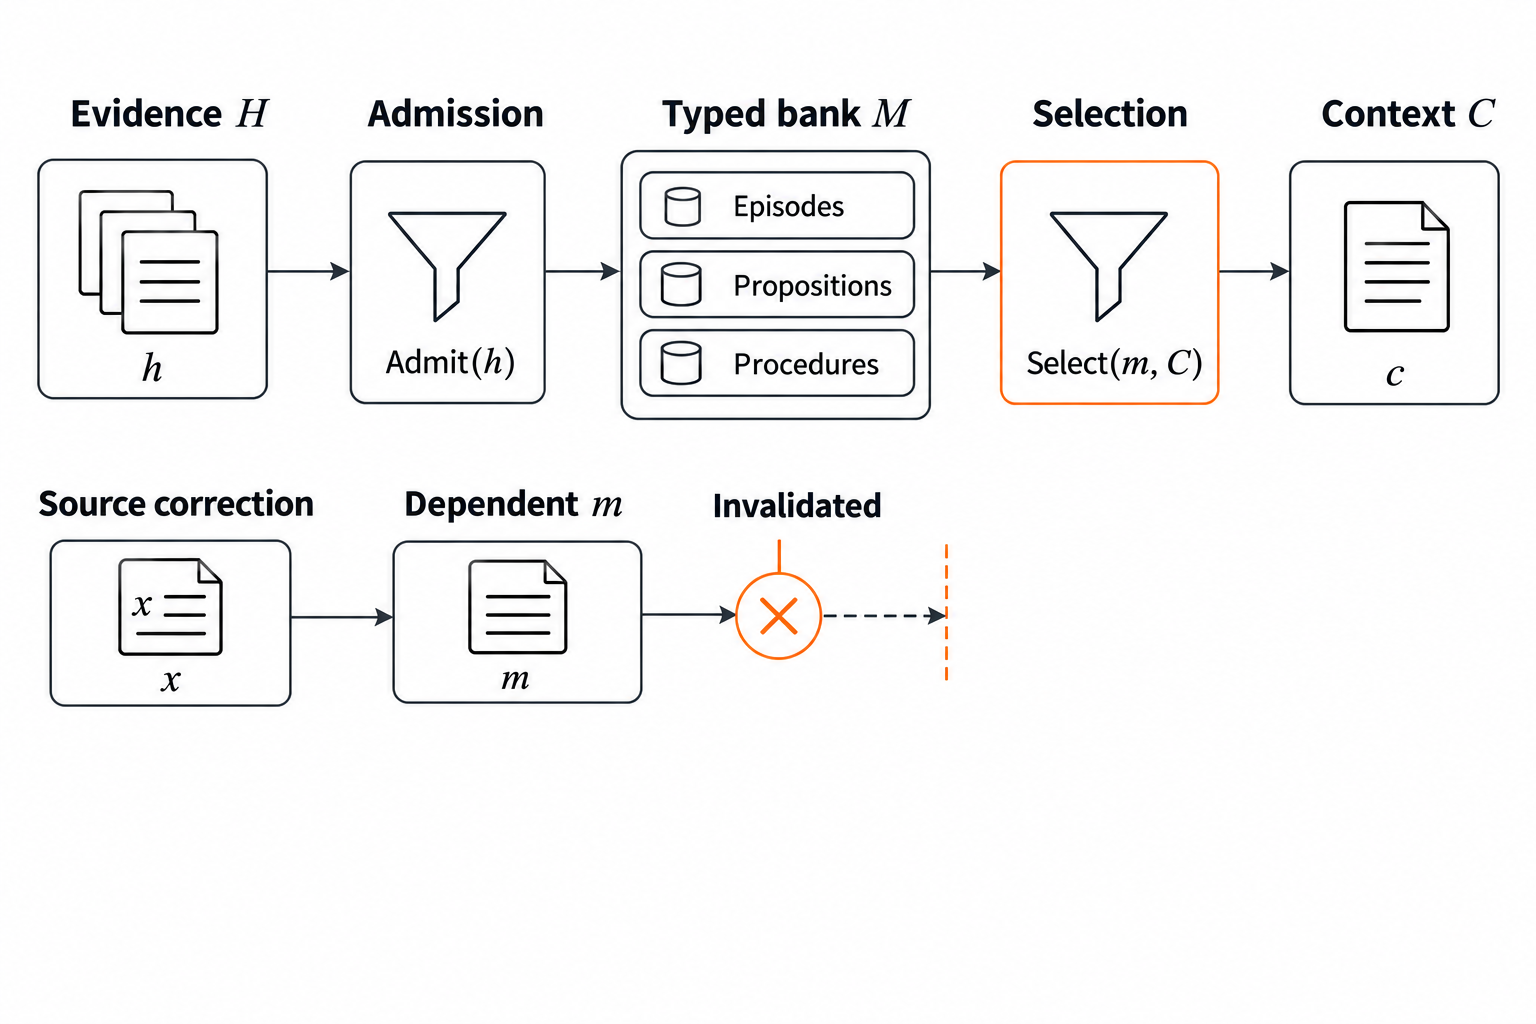
\includegraphics[width=\linewidth]{book/figures/assets/F14review.png}
\caption{Typed retention and invalidation. Evidence $h$ from history $H$ is admitted into a bank $M$ of episodic, propositional and procedural objects. Selection supplies working context $c$; an invalidated dependent object $m$ is blocked pending its specified revalidation. Publication status and provenance remain part of each object record. Current authorization is a separate boundary omitted here. Arrows show lifecycle dependencies, not guaranteed truth or universal conversion between classes. Here $C$ names the working-context component and $c$ its constructed content.}
\label{fig:C14:overview}
\end{figure}
